\begin{center}
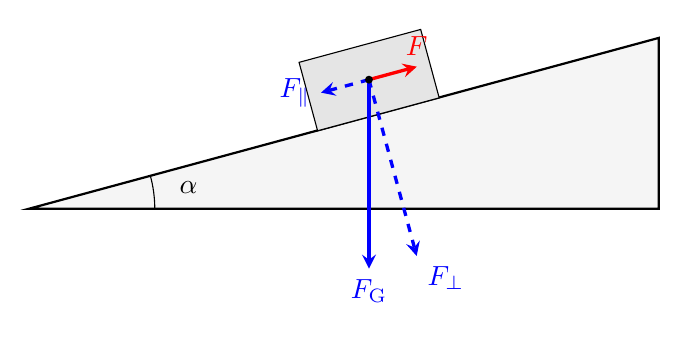
\begin{tikzpicture}[>=stealth]
 \draw[thick, fill=gray!8] (0,0) -- (8.00,0) -- (8.00,2.17) -- cycle;
 \draw (1.6,0) arc (0:15.15:1.6);
 \node at (2.03,0.27) {$\alpha$};
 \begin{scope}[shift={(4.44,1.20)}, rotate=15.15]
  \draw[fill=gray!20] (-0.8,0) rectangle (0.8,0.9);
 \end{scope}
 \draw[->, very thick, blue] (4.32,1.64) -- ++(-90.00:2.40) node[anchor=north] {$F_\mathrm{G}$};
 \draw[->, very thick, blue, dashed] (4.32,1.64) -- ++(-74.85:2.32) node[anchor=north west] {$F_\perp$};
 \draw[->, very thick, blue, dashed] (4.32,1.64) -- ++(195.15:0.63) node[anchor=east] {$F_\parallel$};
 \draw[->, very thick, red] (4.32,1.64) -- ++(15.15:0.63) node[anchor=south] {$F$};
 \fill (4.32,1.64) circle (0.05);
\end{tikzpicture}
\end{center}

Der Rollwagen rollt praktisch reibungsfrei. Die Haltekraft $F$ ist deshalb gleich gross wie die Hangabtriebskraft $F_\parallel = \FPaO$, und die Kraft senkrecht zur Unterlage ist $F_\perp = \FSkO$. Die beiden Komponenten bilden mit der Gewichtskraft ein rechtwinkliges Dreieck, in dem $F_\parallel$ dem Neigungswinkel gegenüberliegt:
\begin{align}
 \tan\alpha &= \frac{F_\parallel}{F_\perp} \\
 \alpha &= \wiF = \arctan\left(\frac{\FPa}{\FSk}\right) = \wi \approx \result{\wiP{0}{2}}
\end{align}
Die Gewichtskraft ist die Hypotenuse des Dreiecks, die Masse also
\begin{align}
 m &= \frac{F_\mathrm{G}}{g} = \mKiF \\
   &= \frac{\sqrt{\left(\FPa\right)^2+\left(\FSk\right)^2}}{\gE} \\
   &= \mKi \approx \result{\mKiP{0}{2}}
\end{align}
